\documentclass{sigchi}

% Use this command to override the default ACM copyright statement (e.g. for preprints). 
% Consult the conference website for the camera-ready copyright statement.


% Arabic page numbers for submission. 
% Remove this line to eliminate page numbers for the camera ready copy
%\pagenumbering{arabic}



\usepackage{balance}  % to better equalize the last page
\usepackage{graphics} % for EPS, load graphicx instead
\usepackage{times}    % comment if you want LaTeX's default font
\usepackage{url}      % llt: nicely formatted URLs
\usepackage{graphicx}
\usepackage{caption}
\usepackage{subcaption}
\usepackage{array}
\usepackage{amsmath}
%\usepackage{multirow}

% llt: Define a global style for URLs, rather that the default one
\makeatletter
\def\url@leostyle{%
  \@ifundefined{selectfont}{\def\UrlFont{\sf}}{\def\UrlFont{\small\bf\ttfamily}}}
\makeatother
\urlstyle{leo}


% To make various LaTeX processors do the right thing with page size.
\def\pprw{8.5in}
\def\pprh{11in}
\special{papersize=\pprw,\pprh}
\setlength{\paperwidth}{\pprw}
\setlength{\paperheight}{\pprh}
\setlength{\pdfpagewidth}{\pprw}
\setlength{\pdfpageheight}{\pprh}

% Make sure hyperref comes last of your loaded packages, 
% to give it a fighting chance of not being over-written, 
% since its job is to redefine many LaTeX commands.
%\usepackage[pdftex]{hyperref}
%\hypersetup{
%pdftitle={L@S 2014 Work-in-Progress Format},
%pdfauthor={LaTeX},
%pdfkeywords={SIGCHI, proceedings, archival format},
%bookmarksnumbered,
%pdfstartview={FitH},
%colorlinks,
%citecolor=black,
%filecolor=black,
%linkcolor=black,
%urlcolor=black,
%breaklinks=true,
%}

% create a shortcut to typeset table headings
\newcommand\tabhead[1]{\small\textbf{#1}}

\begin{document}

\title{Making the Grade}
\large

\numberofauthors{2}
\author{
  \alignauthor Casey O'Brien\\
    \email{cmobrien@mit.edu}
\alignauthor Adam Yedidia\\
\email{adamy@mit.edu}
}

\maketitle

\renewcommand*{\arraystretch}{1.5}

\section{Introduction}

Say that you are a student in a large introductory class, like 6.006. Halfway through the semester, you'd really like to know: \textit{How likely is it that I get an A in this class?}

As TA�s for 6.006, we field questions like this all the time. We answer them with a very practiced response, something like: \textit{We cannot make any predictions about final grades before all assignments are graded}. We say this because we do not want to risk making an incorrect prediction and having the student complain at the end of the semester. However, this is basically a blatant lie. In fact, we think that given a student's grades halfway through the semester, we can make a fairly accurate prediction as to what their final grade in the course will be.

Our work will focus on 6.006, \textit{Introduction to Algorithms}. For the past five years, very little about the class has changed. Each semester, there are 9 assignments: 6 problem sets, 2 quizzes, and a final exam. A student's final numerical grade is weighted as 5\% per problem set, 20\% per quiz, and 30\% for the final exam.

There are three different types of problem that we will discuss in this paper.
\begin{enumerate}
\item \textit{Numerical Prediction}: Predict the student's final numerical average.
\item \textit{Letter Prediction}: Predict the student's final letter grade.
\item \textit{Letter Distribution}: Find the probability distribution over a student's final letter grade.
\end{enumerate}

We solved all of these problems at each point throughout the semester (i.e., after each assignment was due). This allowed us to see how our predictive power increased as we progressed throughout the semester. As one might expect, we saw the largest decreases in our error rates after each of the quizzes.

To compute the numerical prediction, we used regression. For letter prediction, we tried two different models. The first was to perform regression, and then map numerical scores to letter grades. The second was to use an ordered logit/probit model, which, in turn, solved the letter distribution problem. Inspired by the the way that ordered logit/probit computed distributions over the data, we came up with a method for solving the letter distribution problem based on the solution to the numerical predication problem. These models will be discussed in more detail in the coming sections.

\subsection{Data}

We have grade data for six semesters of 6.006 over the past five years. For each student, we have their grade on each assignment, as well as their final letter grade in the class. Within any semester, professors used hard thresholds for letter grade divides. So, if Alice and Bob took 6.006 in the same semester, and Alice had a higher weighted average than Bob, then Alice's letter grade must be at least as good as Bob's.

Figure 1 displays information about our dataset. In particular, Figure 1(a) shows the distribution of students over the different majors (note that double majors were counted in both corresponding columns). We can see that almost all students are either courses 6 or 18. Figure 1(b) shows the gender distribution (which is about 2:1 male:female). Figure 1(c) shows the year distribution, where we see that the students are mostly sophomores. Finally, Figure 1(d) shows the distribution over final grades, which is about 41\% A's, 41\% B's, and 18\% C's. Because the number of $D$'s and $F$'s was so sparse, we considered them the same as $C$'s. So, throughout this paper, $C$'s actually refers to $C$'s, $D$'s, and $F$'s. Note that this distribution varies slightly across different semesters.

\begin{figure*}[t!]

\begin{tabular}{c c c}
\multicolumn{3}{ c }{
	\begin{subfigure}[b]{7in}
		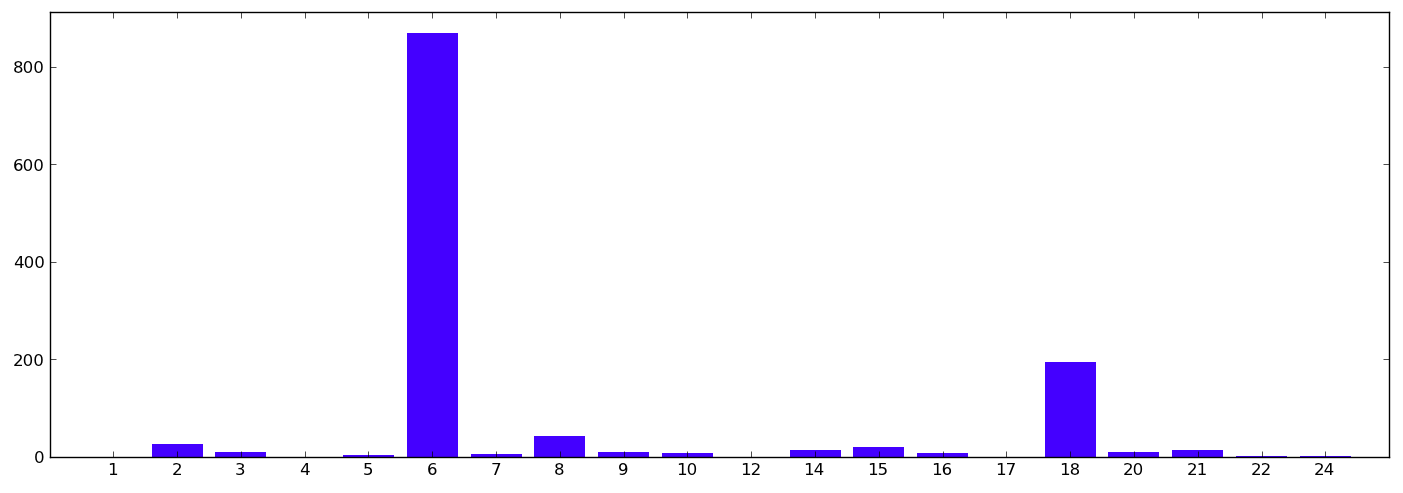
\includegraphics[width=7in]{plots/major.png}
		\caption{The major distribution. Double majors are counted in both columns.}
	\end{subfigure}
	}
\\ &&\\
\begin{subfigure}[b]{2.25in}
	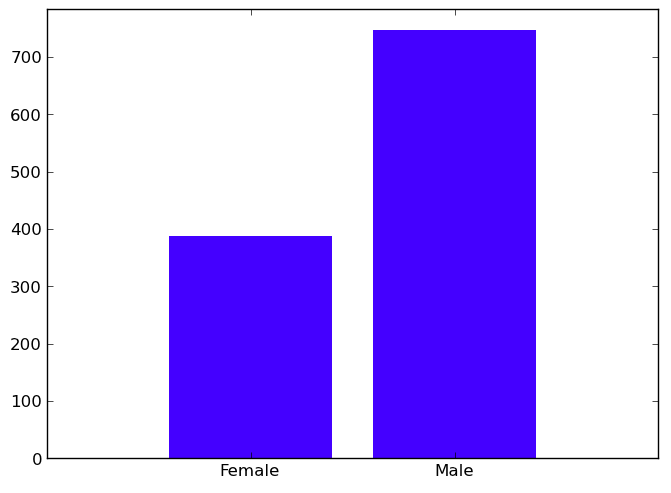
\includegraphics[width=2.25in]{plots/gender.png}
	\caption{The gender distribution.}
\end{subfigure}
&
\begin{subfigure}[b]{2.25in}
	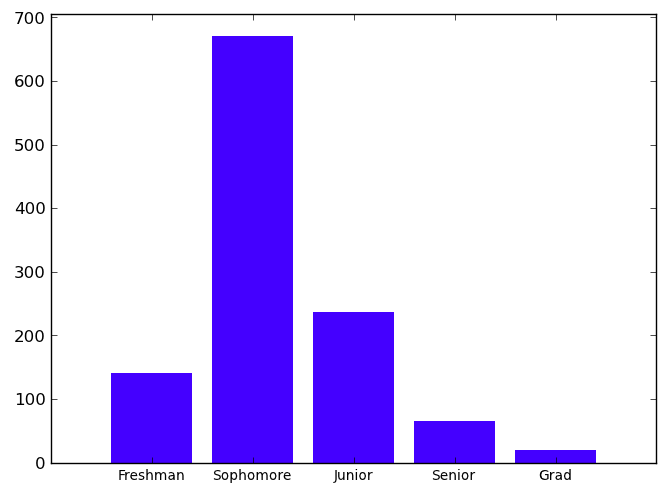
\includegraphics[width=2.25in]{plots/year.png}
	\caption{The class year distribution.}
\end{subfigure}
&
\begin{subfigure}[b]{2.25in}
	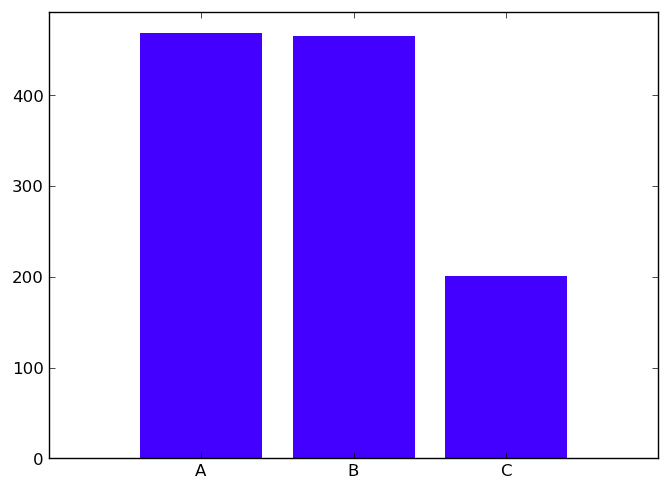
\includegraphics[width=2.25in]{plots/grade.png}
	\caption{The grade distribution.}
\end{subfigure}
\end{tabular}

\caption{Each subfigure shows the distribution over some personal information about the students in our data set. We can see that students are primarily sophomore males in course $6$, and most receive an $A$ or $B$ in the class.}

\end{figure*}

We would like for our models to be able to predict scores not just in these six semesters, but in future semesters. When this is being used in the future, the test data will consist of students from a single semester, and the goal will be to predict their final grades before we actually know them. As such, we randomly chose a single semester of the six to represent our test data. The test data consists of 196 students. The other five semesters, consisting of 938 students in total, were combined and used as training and validation data.

\subsection{Features}

The first, most obvious features to include were the assignment grades. For each assignment (of the assignments being considered at the time), we included as a feature the difference between the student's score and the mean.  We considered dividing by the standard deviation of the assignment (to get the $z$-score), but we realized this has a key flaw. The weighted sum of the $z$-scores of assignments is not equal to the $z$-score of the weighted sum of raw scores. The result is that when students are sorted by weighted sum of $z$-scores, we no longer have the property that grades obey hard thresholds, as described above.

This is perhaps an interesting issue to consider about the way that we assign grades. Say that Alice scores 20 points below average on a test with a very high variance and 20 points above average on a test with very low variance. Bob, on the other hand, scores 20 points above average on the high variance test and 20 points below average on the low variance test. It seems clear that Alice is performing better in the class, yet by our current grading scheme, both students have the same overall score.

Of course, since all of the semesters for which we have data were not graded using $z$-scores, we do not consider this idea any further here.

In order to make it easier to comprehend the weights resulting from our models, we scaled problem set features to be out of 5 (before subtracting the mean), quiz features out of 20, and the final feature out of 30. The result is that when we compare the weights for say, a problem set and a quiz, we can directly compare the effects of a $1\%$ change to final score caused by a problem set and a $1\%$ change to final score caused by a quiz.

Another feature we included is the number of zeros scored on problem sets. For various reasons, some students do not complete certain problem sets throughout the semester. If we are told that a student has an average of $50\%$ on problem sets after the first two problem sets, we might expect that their future problem set scores be about $50\%$. However, if we know that their first problem set score was a $0\%$ and their second a $100\%$, we probably expect their future problem set scores to be much higher than $50\%$.

We also included a feature indicating whether the student took the class in the fall or the spring. While we would not expect to see a huge weight corresponding to this feature, it is interesting to see how it affects our predictions.

For the remainder of our features, we included personal data about the students. To obtain this information, we wrote a web scraper to pull the information from the MIT Alumni Database and MIT People. For each student, we recorded their gender, graduation year, and major.

For five students, we were unable to locate their information. For these students, we guessed their gender (with fairly high confidence) based on their names, and assigned their graduation year and major based on the most likely values. We could have used a more sophisticated method here, but because there were so few students in question, it would have been very unlikely to make any difference.

To capture their gender in a feature, we included a binary variable indicating if the student was male. To capture their graduation year, we included a feature containing the undergraduate school year in which they took the class (e.g., 1, 2, 3, or 4). The few graduate students in the class were considered a 5. Finally, to capture major, we included three binary features, indicating if the student was course 6, course 8, or course 18. Students with double majors had both corresponding features on. While we would have liked to consider the binary features for all other majors, the data was too sparse for us to believe we could get a real signal from it.

\subsection{Roadmap}

In the next section, we will discuss our implementation of regression, and how it allowed us to solve the numerical prediction and letter prediction problems. In the following section, we will discuss the ordered logit and probit models, and how they solved the letter prediction and letter distribution problems. In the final section, we will present a method for solving the letter distribution problem using the results of the numerical prediction problem.

\section{Regression}

\subsection{Motivation}

Linear regression is a very natural approach for solving the numerical prediction problem. The numerical prediction problem involves predicting a single continuous value (a student's final score) as a function of the student's past grades in the class, and personal information about the student, such as year, gender, and major. Moreover, it seems very plausible that the student's final score depends \emph{linearly} on the feature values. Consider grades, for example; we can separate the effect of previous grades into a direct effect and an indirect effect. The direct effect of past grades on final score represents the fact that higher previous grades give you a better final score simply because the final score is partly based on the previous grades. Plainly, this effect is linear (it says so right in the syllabus!) \\

The indirect effect of past grades on final score represents the fact that one's past performance in the class is predictive of future performance. While it is less obvious that this effect is linear, this seems to us to be the most likely interpretation. Consider: the best prediction of how a student will do in the class in the future, to first order, is how they've done in the past. (In fact, it's roughly this times 2/3, because of regression to the mean; and this estimate, of course, ignores the student's personal information. Assuming that a student's performance on assignments is their ``talent'' plus some additive gaussian noise, and talent is normally distributed in the course, talent will depend linearly on past performance, which implies that future performance will depend linearly on past performance). \\

Students' final scores can't help but depend linearly on binary variables such as gender, or membership in a major. The notion that students' final scores depend linearly on their year, however, is more dubious. One might realistically imagine that being a freshman is different from being a sophomore, junior, or senior, for instance, perhaps because letter grades are hidden for freshmen's first semesters at MIT, or perhaps alternately because taking 6.006 as a freshman signals a particular enthusiasm for the study of algorithms that taking 6.006 as a sophomore, junior, or senior simply might not indicate. \\

We looked at the average scores of freshmen, sophomores, juniors, and seniors, and found that the A/B/C distribution went 61\%/24\%/14\% for freshmen, 44\%/42\%/14\% for sophomores, 32\%/39\%/29\% for juniors, and 30\%/30\%/39\% for seniors. This progression is perhaps not exactly linear; we felt, however, that it was close enough to linear to warrant inclusion of year as a continuous variable in its own right, and not as four binary variables, into our model. \\

Because all of the features have a linear or nearly-linear relationship with the number we seek to predict, linear regression is a good tool to use to solve this problem.

\section{Implementation}

Our implementation uses ridge regression to predict students' numerical final scores as a function of the feature vectors. We make use of the ordinary least-squares method for solving a matrix equation to get the vector of weights, which allows us to map from feature vectors to predicted final score values.

Let $n$ be the number of students in our data set, and let $d$ be the dimensionality of our feature vectors. (If we were doing prediction knowing only the scores on the first three assignments, $d$ would be 8: three features for being course 6, course 8, or course 18, one feature for gender, one feature for year, and one feature for each of the three assignments.) Let $X$ be the $n \times d$ matrix of feature vectors, and let $Y$ be the be the $n \times 1$ vector of true final scores.

%Let $X'$ be the feature matrix, but with 1's (in order to be able to properly calculate the offset $x_0$) prepended to each of the matrix's rows. $X'$ is therefore an $n \times (d+1)$ matrix. \\

Let $Z$ be the \emph{centralized} data matrix; in other words, just as $X$ is a matrix of feature vectors $x^{(i)}$, $Z$ is a matrix of normalized feature vectors $z^{(i)}$, where each vector $z^{(i)}$ is defined in terms of $X$ as follows: 

$$z^{(i)} = x_j^{(i)} - x_j$$

Similarly, we defined a centralized result matrix $Y_c$ with

$$y_c^{(i)} = y^{(i)} - \bar{y}$$

As described in the class notes on regression, the least-squares-optimal value for the weight vector assuming quadratic regularization is given by:

$$w = (Z^T Z + \lambda I)^{-1} Z^T Y_c$$

The offset $w_0$ is in turn given by:

$$W_0 = (\bar{y} - W^T\bar{X})$$

\subsection{Results}

When we ran ridge regression on past semesters' data, we got the following values for the weight vector's entries. Note that we ran the regression after knowing 0, 3, 6, and 9 of the assignments' values, respectively, before predicting final score. 

\begin{figure*}
\centering
\begin{tabular}{c c}
\begin{subfigure}[b]{3in}
	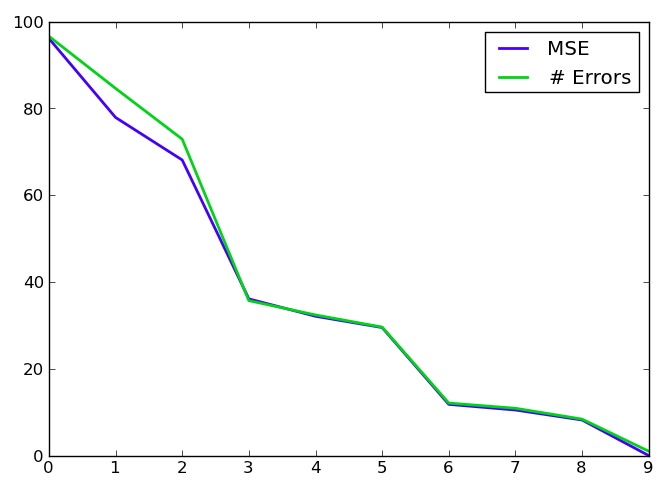
\includegraphics[width=3in]{plots/mse.png}
	\caption{MSE v. number of assignments}
\end{subfigure}
&
\begin{subfigure}[b]{3in}
	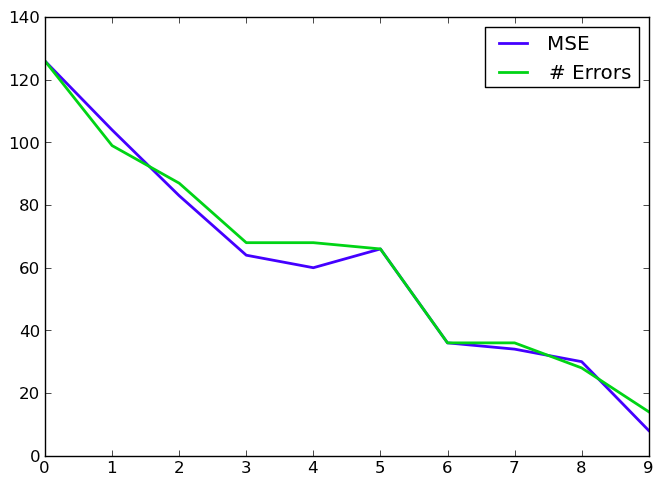
\includegraphics[width=3in]{plots/num_errors.png}
	\caption{Number of errors v. number of assignments}
\end{subfigure}
\\
\begin{subfigure}[b]{3in}
	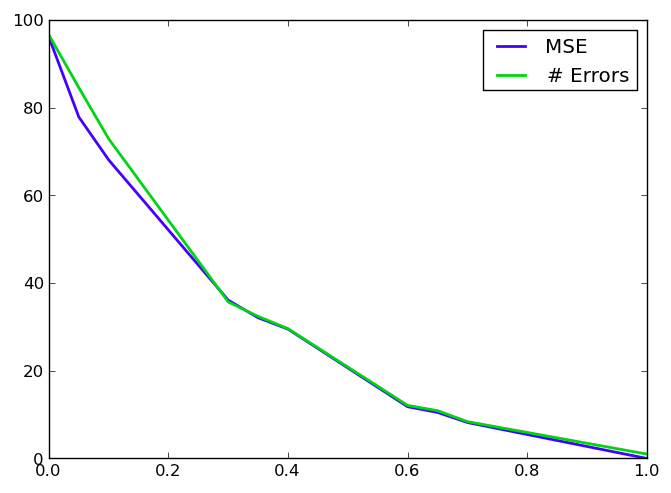
\includegraphics[width=3in]{plots/mse_percentage.png}
	\caption{MSE v. percentage of final grade}
\end{subfigure}
&
\begin{subfigure}[b]{3in}
	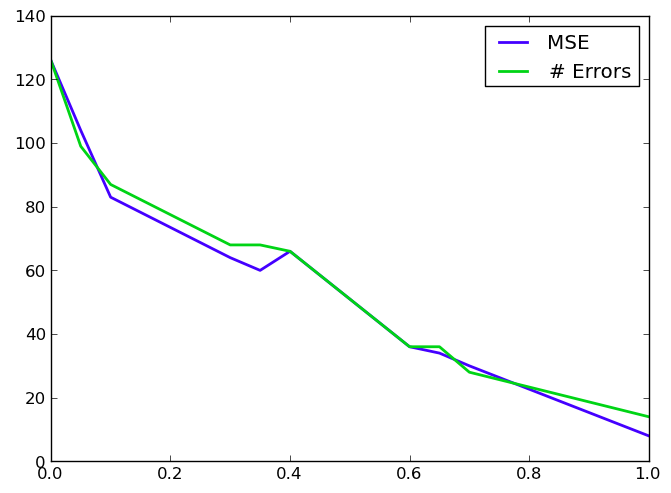
\includegraphics[width=3in]{plots/num_errors_percentage.png}
	\caption{Number of errors v. percentage of final grade}
\end{subfigure}
\end{tabular}
\caption{The left column shows the value of the MSE, while the right column shows the number of errors in the test set. The top row shows these values as a function of the number of assignments included as features, and the bottom rows shows the values as a function of percentage of the final grade included as features. All plots show results for both when we were minimizing MSE and when we were minimizing number of errors.}
\end{figure*}

\begin{figure}
\centering
\begin{tabular}{| c || c | c | c | c |}
\hline
 &\multicolumn{4}{ c |}{Weights}\\
\hline
\# Assignments & 0 & 3 & 6 & 9 \\
\hline
$w_0$ & $5.04$ & $-1.00$ & $-0.07$ & $0.00$ \\ 
\hline
Problem Set 1 & $-$ & $2.44$  & $1.11$  & $1.00$ \\
\hline
Problem Set 2 & $-$ & $4.04$  & $0.85$ & $1.00$ \\
\hline
Quiz 1	      & $-$ & $2.49$  &  $1.53$ & $1.00$ \\ 
\hline
Problem Set 3 & $-$ & $-$          & $1.94$ & $1.00$ \\
\hline 
Problem Set 4 & $-$ & $-$          & $1.99$ & $1.00$  \\
\hline
Quiz 2	       & $-$ & $-$          & $1.79$ & $1.00$ \\
\hline
Problem Set 5 & $-$ & $-$          & $-$& $1.00$\\
\hline
Problem Set 6 & $-$ & $-$          & $-$& $1.00$ \\
\hline
Final		& $-$       & $-$          & $-$& $1.00$\\
\hline
Pset-zeros   & $-$ & $4.89$ & $-0.08$ & $0.00$ \\
\hline
Fall		&  $0.62$     & $0.98$ & $1.49$ & $0.00$ \\
\hline
Male		&  $1.00$     & $1.41$  & $0.26$ & $0.00$ \\
\hline
Year 		&  $-2.82$   & $-1.06$ & $-0.16$ & $0.00$\\
\hline
Course 6	&  $-0.34$    & $1.80$  & $0.03$ & $0.00$ \\
\hline
Course 8	&  $0.45$  &  $1.57$  &  $0.40$  &  $0.00$ \\
\hline
Course 18       & $2.00$ & $2.58$  & $0.17$ & $0.00$ \\
\hline
\end{tabular}
\caption{Each column represents the weights returned by ridge regression with the optimal value of $\lambda$, using the number of assignments specified in the column head as features. }
\end{figure}

Looking at the above results, there are a few noteworthy trends. The first is that weights tend to decrease in absolute value as one progresses across the table from left to right; the weights for assignments tend towards one, and the weights for personal statistics tend towards zero. This is comforting, because the theory we had was that assignments would have weights of more than one and personal statistics would have non-zero weights because both the early assignment scores and the personal statistics have some predictive power over future assignments. As the number of future assignments decreases, then, one would naturally expect this predictive effect to decrease and the direct effect of assignment grades being factored into final grades to increase. \\

In addition to this overall effect on the columns of the table, we can observe some interesting trends no rows. Taking the class in the fall, being male, and being a physics major all appear to give a small advantage in 6.006; being a math major, and being a freshman rather than a junior or a senior both appear to confer a somewhat more important advantage. \\

All of these effects, of course, are dwarfed by the predictive effect of early assignments on later ones. This is entirely unsurprising; as discussed earlier, the best predictor of final score is, to first order, performance up until this point. \\

There is one more feature that deserves mention here, and that is the effect on score of getting zeros on problem sets. We theorized early on that getting zeros on problem sets would actually have a substantial \emph{positive} effect on predicted score, because a zero on a problem set does not carry the same predictive weight that poor scores on assignments otherwise might. Put otherwise, most low scores on assignments tend to signal a relatively poor understanding of the material, whereas a zero on a problem set might instead be signaling simple laziness. We see that this theory is more or less borne out by the data, with the positive effect of problem set zeros beginning strong and quickly becoming very weak as the predictive effect of problem sets diminishes with time.

\subsection{Predicting Letter Grades}

As noted above, regression is extremely well-suited to predicting numerical scores. Predicting letter grades, however, is perhaps a slightly more awkward fit, since linear regression is not properly designed for classification. \\

In order to use linear regression to predict letter grades, the simplest conversion is simply to take the predicted final scores returned by the ridge regression as described above, and sort the scores into A, B, and C bins according to the average number of A's, B's, and C's given out in a given semester. \\

In other words, suppose that in an average run of 6.006, the distribution of grades is 40\% A's, 40\% B's, and 20\% other grades, abbreviated in this paper as ``C's.'' (In reality, the average run of 6.006 has slightly more A's and slightly fewer C's than that, but it's close enough.) In that case, we take the final scores predicted by the ridge regression, and we assign the predicted scores of the students to letter grades according to whether they belong to the top 40\% of predicted scores (in which case we predict an A), the bottom 20\% of predicted scores (in which case we predict a C) or the middle 40\% of predicted scores (in which case we predict a B). Call this mapping from numerical scores $s$ to letter grades $c(s)$\\

If we just do this--take the weights from the previous section that were designed to minimize MSE between predicted final score and actual final score, and use them to classify students by grade--we do reasonably well, misclassifying 8 students when we have access to every assignment grade and 126 students when we have access to none of them. The misclassification rate of this algorithm is illustrated in more detail in the figure below. \\ % TODO deal

However, this approach is somewhat unnatural, in that the weight vector is being optimized to minimize MSE, but is being used to predict letter grades. It would seem to make more sense to optimize the weight vector to minimize the number of errors in letter grade classification, if that is what it is going to eventually be used for. Therefore, we seek to minimize the following error function:

$$E(w) = \sum_i e^{(i)} + \lambda ||w||^2$$

where $e^{(i)} = 1$ if $c(x^{(i)} \cdot w) = y^{(i)}$ and $e^{(i)} = 0$ if $c(x^{(i)} \cdot w) \not{=} y^{(i)}$, with $c(s)$ defined as above.    \\

This error function is not nicely differentiable the way the ordinary goal function for ridge regression is. Therefore, we could not find a closed form for the solution; instead, we performed a gradient descent over the $w$ values, in an attempt to find a local minimum whose values will hopefully not be far from those of the global minimum. To do this gradient descent, we used the fmin_bfgs package from scipy.\\

To our mild surprise, the results of the gradient descent did not yield materially different results from the MSE minimization, either in terms of the observed mean-squared-error (which would have expected the previous method to perform better at) or in terms of the number of errors in classification in the test set (which we would have expected the previous method to perform worse at). The new method misclassified 14 students with access to every assignment grade and 126 students with access to no assignment grades. A more complete description of its performance is visible in the figure below. % TODO deal

\section{Ordered Logit/Probit}

This problem seems to lend itself more naturally to classification than to regression. Thus, we decided to model this problem as a classification problem. Now, we are no longer interested in predicting students' final numerical scores. Instead, we are only interested in predicting students' final letter grade.

Given a student's grades and information partway through the semester, we want to predict their final letter grade. This can easily be modeled as a multi-class classification problem. However, the problem is actually more structured than that, because our class values, $A$, $B$, and $C$, have an inherent ordering. Thus, we make use of ordered logit and ordered probit.

These techniques are very similar, so at first we will not differentiate between them. The goal is to map the feature vector, which we will call $x$ for simplicity, to a real number. We will do this by solving for a weight vector $w$, and then mapping $x$ to $x \cdot w$. Then we want to choose cutoffs $\mu_A$ and $\mu_B$ which separate the $A$'s, $B$'s and $C$'s. Once we have solved for $w$, $\mu_A$, and $\mu_B$, we can predict a final grade $y$ as follows

\begin{equation} y=
\begin{cases} 
      A &  \mu_A \leq x \cdot w\\
      B & \mu_B \leq x \cdot w < \mu_A \\
      C & x \cdot w < \mu_B 
   \end{cases}.
\end{equation}

Note the lack of $w_0$ term above. We can see that if we chose to include a $w_0$ term, it would simply result in each $\mu$ being offset by $w_0$ as well, leading to an equivalent result. Thus, without limiting our model, we can omit $w_0$.

\subsection{Ordered Probit}

We will first describe the ordered probit model. Say that we assume that a student's final score will be distributed as a Gaussian around their current scores with standard deviation $\sigma$. If we knew the thresholds $\mu_A$ and $\mu_B$, we could calculate the probability that a student received an $A$ in the class as
\[P(y = A) = \Phi \left (\frac{x \cdot w - \mu_A}{\sigma} \right ).\]
Similarly, we have
\begin{equation*}
\begin{split}
P(y = B) & = \Phi \left ( \frac{\mu_A - x \cdot w}{\sigma} \right ) - \Phi \left (\frac{\mu_B - x \cdot w}{\sigma} \right ) \\\
P(y = C)  &= \Phi \left (\frac{\mu_B - x \cdot w}{\sigma} \right ).
\end{split}
\end{equation*}
From these equations, it is easy to see that if $x \cdot w > \mu_A$, then $P(y = A) > P(y = B) > P(y = C)$. So, whenever we have $x \cdot w > \mu_A$, the maximum likelihood estimate will be $A$. Using similar reasoning for when $x \cdot w < \mu_A$, we can see that equation (1) is simply saying to choose the maximum likelihood estimate.

This works out nicely, but we still need to solve for $w$, $\mu_A$, and $\mu_B$, and now $\sigma$ as well. First, we note that we can set $\sigma = 1$, and it will not restrict our model at all, as we can scale $w$, $\mu_A$, and $\mu_B$ accordingly. So now we have
\begin{equation*}
\begin{split}
P(y = A) &= \Phi \left (x \cdot w - \mu_A \right )\\
P(y = B) &= \Phi \left (\mu_A - x \cdot w \right ) - \Phi \left (\mu_B - x \cdot w \right )\\
P(y = C) &= \Phi \left (\mu_B - x \cdot w \right ).
\end{split}
\end{equation*}
Of all the students that we eventually assign an $A$, we would like to maximize the likelihood that they receive an $A$, and similarly for $B$'s and $C$'s. So, our goal will be to solve the following optimization:
\[\max_{w, \mu_A, \mu_B} L(w, \mu_A, \mu_B),\]
where
\begin{equation*}
\begin{split}
L(w, \mu_A, \mu_B) &= \prod_{\hat{y}^{(i)} = A} P(y = A)\\
&\times \prod_{\hat{y}^{(i)} = B} P(y = B)\\
&\times \prod_{\hat{y}^{(i)} = C} P(y = C)
\end{split}
\end{equation*}
To solve this problem, we instead try to minimize the negative log-likelihood. So, our optimization problem is now
\[\min_{w, \mu_A, \mu_B} -\log{L(w, \mu_A, \mu_B)},\]
where
\begin{equation}
\begin{split}
-\log{L(w, \mu_A, \mu_B)} =& -\sum_{\hat{y}^{(i)} = A} \log{P(y = A)}\\
&- \sum_{\hat{y}^{(i)} = B} \log{P(y = B)}\\
&- \sum_{\hat{y}^{(i)} = C} \log{P(y = C)}.
\end{split}
\end{equation}

\subsection{Ordered Logit}

The ordered logit model is very similar to the ordered probit model. The difference is that instead of assuming that future grades are distributed as a Gaussian, we assume that they are distributed according to a logistic distribution. Figure xx shows the differences between the Gaussian distribution and the logistic distribution. A logistic distribution is something like a Gaussian distribution with ``fat tails''.

\begin{figure*}
\centering
\begin{tabular}{c c}
\begin{subfigure}[b]{3in}
	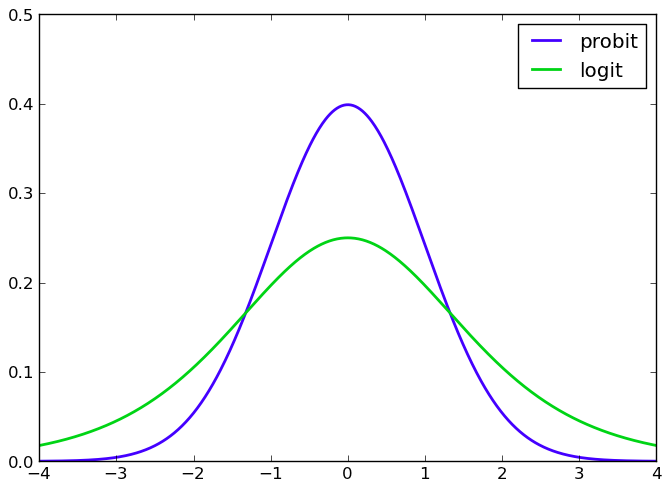
\includegraphics[width=3in]{plots/pdf.png}
	\caption{PDF}
\end{subfigure}
&
\begin{subfigure}[b]{3in}
	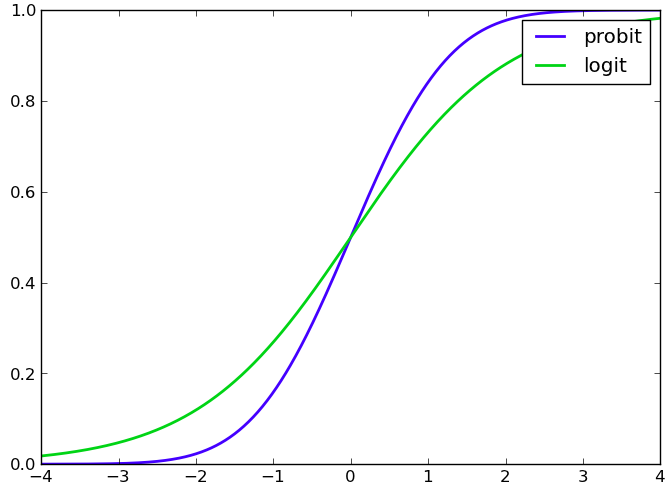
\includegraphics[width=3in]{plots/cdf.png}
	\caption{CDF}
\end{subfigure}
\end{tabular}
\caption{The CDF and PDF of Gaussian and logistic distributions with mean $0$ and standard deviation $1$.}
\end{figure*}

The cumulative distribution function for the logistic distribution is given by
\[F(x) = \frac{1}{1 + e^{-x}}.\]
Thus, to perform ordered logit, we simply need to replace occurrences of $\Phi$ in ordered probit with $F$. So now we have
\begin{equation*}
\begin{split}
P(y = A) &= F \left (x \cdot w - \mu_A \right )\\
P(y = B) &= F \left (\mu_A - x \cdot w \right ) - F \left (\mu_B - x \cdot w \right )\\
P(y = C) &= F \left (\mu_B - x \cdot w \right ).
\end{split}
\end{equation*}
From here, the form of equation xx is unchanged.

\subsection{Choosing a Model}

It's difficult to tell which of the ordered probit or logit models will be more suitable for the data. It depends on knowing how future student grades depend on past student grades. To get a sense for this distribution, we graphed it.

Consider the point in the semester after which we know 3 student grades (two problem sets and a quiz). For each student in the training set, we computed our best guess of their average at that point in the semester (using ridge regression). We then subtracted their final numerical average in the class. The result is the amount that their average changed. Figure xx shows histograms of these values at the beginning of the semester, after 3 assignments, after 6 assignments, and after 9 assignments.

\begin{figure}
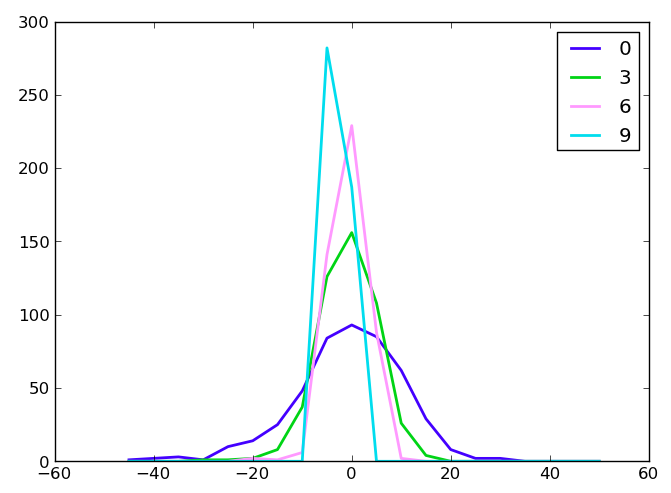
\includegraphics[width = 3in]{plots/gaussian.png}
\caption{The distribution over differences between final grades and predicted grades. Each curve corresponds to a different number of assignments used as features to compute the predicted grades.}
\end{figure}

The distributions seem relatively Gaussian, with smaller standard deviations as the semester progresses. This is what we would expect, since later in the semester, much less of the grade is unknown. We also notice that the curves tend to be centered slightly to the left of the origin.

For 6.006, almost all assignment averages are above $50\%$. As a result, it is possible to fail by more than it is possible to succeed. Histograms of assignments tend to be skewed to the right. Our model does not take advantage of this trend.

Clearly, the graph does not contain enough information for us to distinguish between a Gaussian and a logistic distribution. As such, we will apply both ordered logit and ordered probit to our data.

\subsection{Applying To Our Data}

To solve these optimization problems, we implemented ordered logit and probit in Python, by minimizing the objective functions using \texttt{fmin\_bfgs}.

Because ordered logit and probit do not have any parameters we need to use validation data to optimize, for this section we combined our training and validation data, so that our training set has 938 points.

Next, we applied these models to our data in order to predict student letter grades. As before, we applied both of these models after each assignment throughout the semester. The results were very similar to those described in the Regression section.

\begin{figure}
\centering
\begin{subfigure}[b]{3in}
	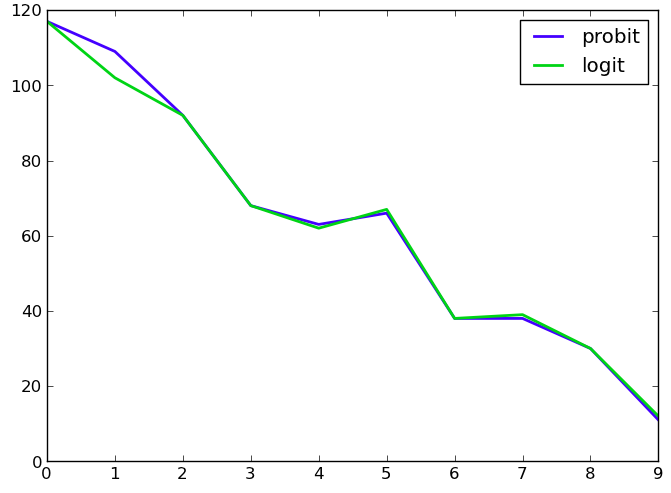
\includegraphics[width=3in]{plots/ordered_num_missed.png}
	\caption{Number of errors v. number of assignments}
\end{subfigure}
\begin{subfigure}[b]{3in}
	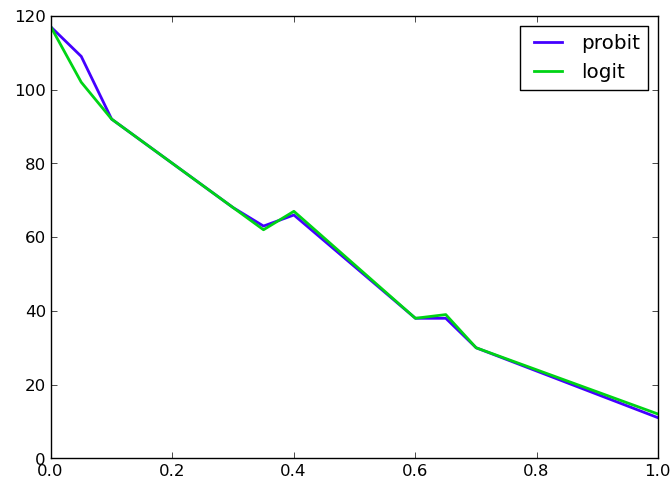
\includegraphics[width=3in]{plots/percentage_num_missed.png}
	\caption{Number of errors v. percentage of final grade}
\end{subfigure}
\caption{Depicts the test error as we increase the number of assignments that we include as features. Each graph shows the results using each of the ordered logit and ordered probit models.}
\end{figure}

Figure xx(a) shows the number of misclassified students as a function of the number of assignments included as features. To properly read this graph, keep in mind the order of assignments:
\[PS1, PS2, Q1, PS3, PS4, Q2, PS5, PS6, F\]
We are not surprised to see that we see the largest drops in number of misclassified students after the third, sixth, and ninth assignments, as these assignments make up the largest proportions of student grades.

This graph is slightly misleading, as it should obviously be the case that the assignments which make up the largest percentages of their grades give us the most information. In Figure xx(b), we see the same curves, but plotted against the percentage of the final grade which had been determined after that assignment.

After the first quiz, students have only completed 30\% of their final weighted grade. Even at this point in the semester, we are able to classify student's final grades with 65\% accuracy. After the second quiz, when 60\% of the final grade is determined, we are able to classify student grades with 81\% accuracy. After the final, when 100\% of the final grade is determined, we classify student grades with 94\% accuracy.

We notice that the amount that our error decreases is not quite linear in the number of percentage points which we include in the features. This implies that as we know more about student grades, each additional percentage point tells us less information than the previous. It is also interesting to note that problem set percentage points improve our predictions by just as much as quiz percentage points. In other words, the amount by which our error decreases after a problem set appears to be about one-quarter the amount by which our error decreases after a quiz.

Note that the most common grade among the training data was a $B$. Thus, we can compare these results to the case where we assign $B$'s to all students in the class. This would result in a test error of 122 (corresponding to a 37.8\% accuracy rate), which is slightly worse than that achieved by ordered logit/probit, even when no assignments are considered. Thus, using just personal information about the students, we are able to do better than the trivial algorithm.


It is somewhat disappointing that we are not able to determine final grades with 100\% accuracy, even when all of their scores are completely determined. The reason for this is variation among thresholds from different professors. If professors observed strict proportions of $A$'s, $B$'s, and $C$'s, we could easily predict grades with 100\% accuracy after the final. Sadly, MIT does not allow such grading policies.

\subsubsection{Feature Weights}

To see how important the models consider the various features, let us look at the weights that they produce for each feature at various points throughout the semester.

Figure 3 shows the weights assigned to each feature after 3, 6, and 9 assignments (note that these mark the points after each quiz/final) for ordered probit. We can observe some general trends from looking at these weights. First, the assignment scores tend to carry a lot more weight than the personal information, which is expected.

The weights of all the assignments tend to be very similar. Recall that the values of the features already take into account the fact that different assignments have different weights in their final grades, so we expect these weights to be roughly equal.

We do see some variety among the weights, although we believe this is because there is some noise introduced by the fact that these assignments had different variances (and the variances differed slightly among years). For example, most students perform very well on problem set 1. Thus, a student's score on problem set 1 does not give us much information about their final grade. We believe this is why we tend to see a much lower weight on the first problem set. 

\begin{figure}
\centering
\begin{tabular}{| c || c | c | c | c |}
\hline
 &\multicolumn{4}{ c |}{Weights}\\
\hline
Feature & 0 & 3 & 6 & 9 \\
\hline
\hline
Problem Set 1 & $-$ & $0.17$  & $0.16$  & $0.36$ \\
\hline
Problem Set 2 & $-$ & $0.45$  & $0.23$ & $0.46$ \\
\hline
Quiz 1	       & $-$ & $0.49$  &  $0.45$ & $0.49$ \\ 
\hline
Problem Set 3 & $-$ & $-$          & $0.53$ & $0.44$ \\
\hline 
Problem Set 4 & $-$ & $-$          & $0.39$ & $0.30$  \\
\hline
Quiz 2	       & $-$ & $-$          & $0.38$ & $0.35$ \\
\hline
Problem Set 5 & $-$ & $-$          & $-$& $0.62$\\
\hline
Problem Set 6 & $-$ & $-$          & $-$& $0.28$ \\
\hline
Final		       & $-$ & $-$          & $-$& $0.50$\\
\hline
Problem Set $0$'s & $-$ & $-0.39$ & $-0.16$ & $0.04$\\
\hline
Fall		       & $0.051$ & $-0.08$ & $-0.20$ & $-0.23$ \\
\hline
Male		       & $0.014$ & $0.07$  & $0.00$ & $0.05$ \\
\hline
Year 		       & $-0.27$ & $-0.10$ & $0.00$ & $0.01$\\
\hline
Course 6	       & $0.17$ & $0.28$  & $0.19$ & $0.49$ \\
\hline
Course 8	       & $0.71$ & $0.26$  & $0.49$ & $0.00$ \\
\hline
Course 18       & $0.13$ & $0.34$  & $0.10$ & $0.15$ \\
\hline
\end{tabular}
\caption{Each column represents the weights returned by ordered probit with the optimal value of $\lambda$, using the number of assignments specified in the column head as features.}
\end{figure}


\subsubsection{Grade Distributions}

Next, we move on to focus on the grade distribution problem. Note that when we solved the ordered logit/probit, we already solved the grade distribution problem. To solve the grade prediction problem, we simply chose the maximum likelihood estimate. However, this is just throwing away additional information.

Consider a student who comes to you, their TA, after quiz 1, wanting to know what their final grade will be. If you, the TA, predict they will get an $A$, and then they end up with a $B$, they will probably be very unhappy with you at the end of the semester. Instead, if you tell them they have a $52\%$ chance of getting an $A$ and a $48\%$ change of getting a $B$, they will probably by much less angry come the end of the semester.

With this in mind, perhaps finding the number of misclassified students is not the correct function to focus on. In fact, this was not the function that we minimized when we solved the ordered logit/probit problem. Recall that our goal was to minimize the negative log likelihood.

While we chose to minimize the negative log likelihood (as opposed to just maximizing the likelihood), primarily for mathematical convenience, the value of this function has some interesting properties. In some sense, we can think of it as a penalty function for an assignment of distributions. A lower penalty corresponds to a better distribution. 

We notice that if we assign a student a $0\%$ chance of receiving a grade that they eventually receive, then our penalty is $\infty$. This is desirable, because if we are ever so sure that a student has a $0\%$ chance of receiving a grade, and we end up being wrong, our predictor is clearly doing a very poor job (note that our algorithm will never assign a probability of $0\%$, just arbitrarily small probabilities).

We also notice that if we guess their grade correctly with $100\%$ certainly, we suffer no penalty. This also seems appropriate. If we are entirely sure of a student's final grade, then we should not be penalized for our guess.

Figure xx shows the minimum values of the negative log likelihoods after each assignment is due, for both ordered logit and probit. Interestingly, they produce nearly identical results. This is good news, because it means that the distributional assumptions are not driving the result. As in Figure xx, we show both the curves as a function of the number of assignments completed (in Figure xx(a)), and as a function of percentage of the grade completed (in Figure xx(b)). 

In Figure xx(b), we also observe that the value of the slope decreases slightly as we determine more of their final grades. Again, this points to the fact that as we move through the semester, each additional determined percentage point tells us less than the previous.

\begin{figure}
\centering
\begin{subfigure}[b]{3in}
	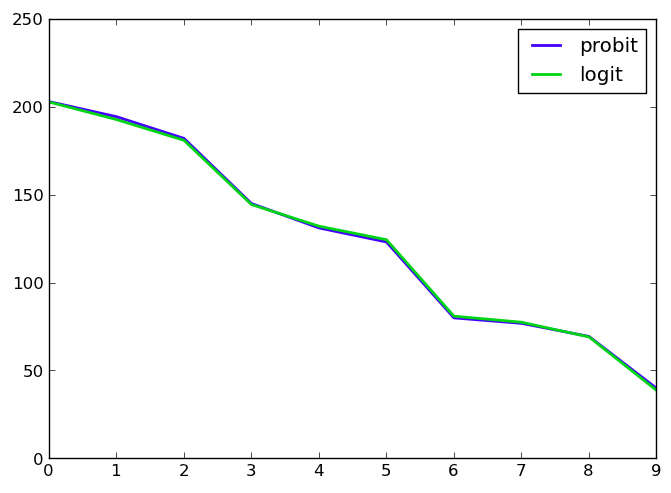
\includegraphics[width=3in]{plots/ordered_score.png}
	\caption{NLL v. number of assignments}
\end{subfigure}
\begin{subfigure}[b]{3in}
	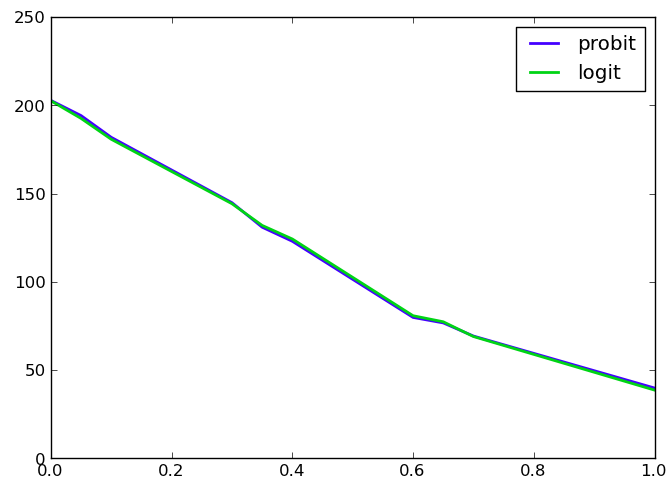
\includegraphics[width=3in]{plots/percentage_score.png}
	\caption{NLL v. percentage of final grade}
\end{subfigure}
\caption{Depicts the value of the minimum negative log likelihood as we increase the number of assignments used as features. Each graph shows the results using each of the ordered logit and ordered probit models.}
\end{figure}

In our training data, we observe $41.0\%$ $A$'s, $41.7\%$ $B$'s, and $17.3\%$ $C$'s. We could trivially assign each student in the test set this probability distribution. In the test set, there are 83 $A$'s, 74 $B$'s, and 39 $C$'s. Using this assignment, the negative log likelihood would be
\[- 83 \cdot \log(0.410) - 74 \cdot \log(0.417) - 39 \cdot \log(0.173)\]
\[ = 207.15\]
Again, we notice that even with no assignments included in the features, our ordered logit/probit is able to do slightly better than the trivial solution.

\begin{figure*}
\centering
\begin{tabular}{c c}
\begin{subfigure}[b]{3in}
	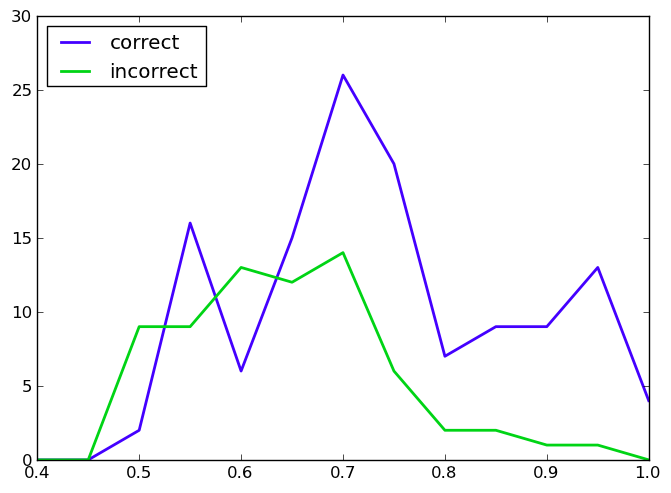
\includegraphics[width=3in]{plots/probit3dist.png}
	\caption{Histogram of ML's for 3 assignments}
\end{subfigure}
&
\begin{subfigure}[b]{3in}
	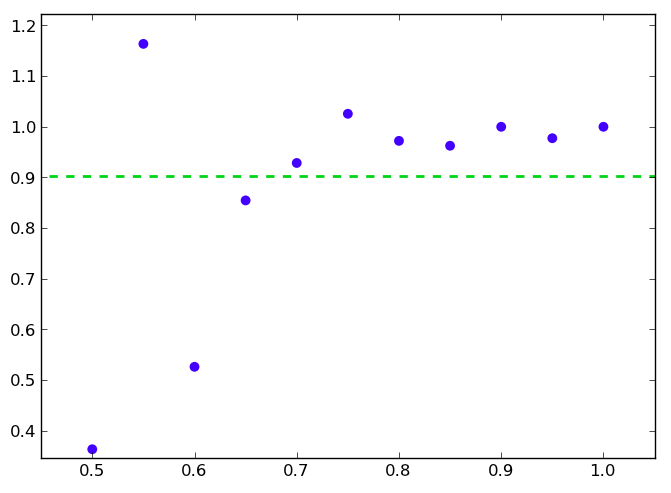
\includegraphics[width=3in]{plots/1pro3.png}
	\caption{Ratio of ML to percentage correct for 3 assignments}
\end{subfigure}
\\
\begin{subfigure}[b]{3in}
	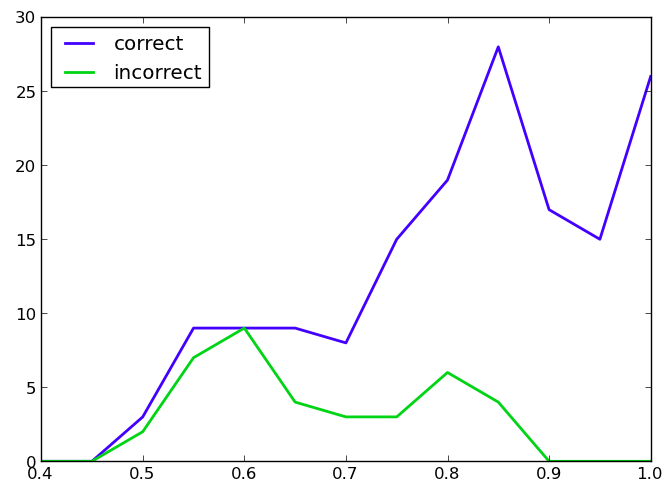
\includegraphics[width=3in]{plots/probit6dist.png}
	\caption{Histogram of ML's for 6 assignments}
\end{subfigure}
&
\begin{subfigure}[b]{3in}
	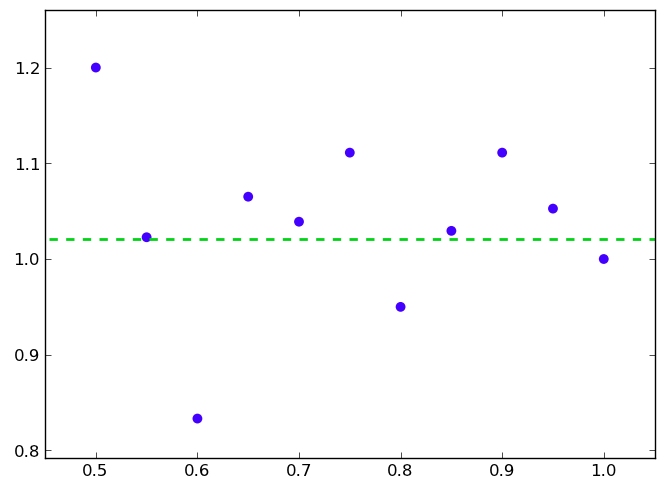
\includegraphics[width=3in]{plots/1pro6.png}
	\caption{Ratio of ML to percentage correct for 6 assignments}
\end{subfigure}
\\
\begin{subfigure}[b]{3in}
	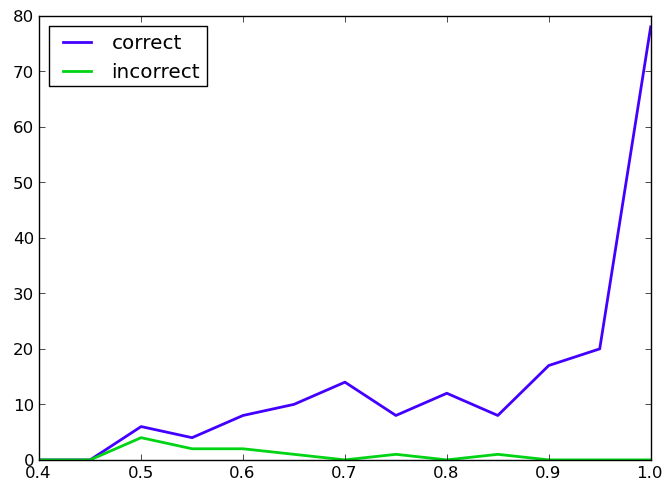
\includegraphics[width=3in]{plots/probit9dist.png}
	\caption{Histogram of ML's for 9 assignments}
\end{subfigure}
&
\begin{subfigure}[b]{3in}
	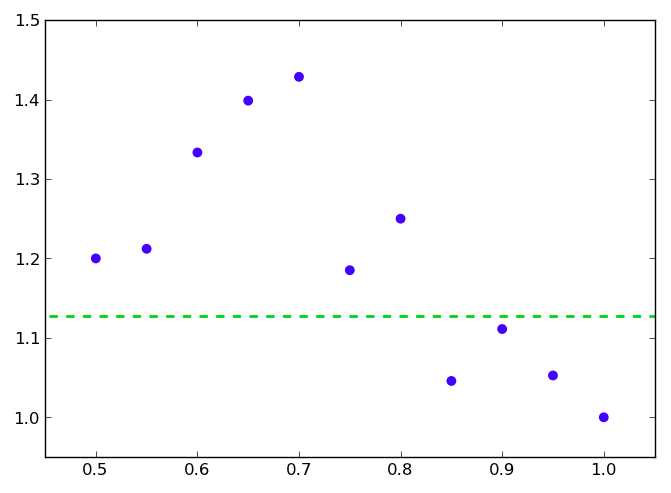
\includegraphics[width=3in]{plots/1pro9.png}
	\caption{Ratio of ML to percentage correct for 9 assignments}
\end{subfigure}
\end{tabular}
\caption{Visualizations of the maximum likelihood values when finding distributions using ordered probit. The left column shows a histogram of students who had a maximum likelihood value (bucketed to 5\%), for both students we could classify correctly and those we couldn't. The right column shows the ratio of the maximum likelihood value to the percentage of students with that value that we could guess correctly. The dotted line show the average, which we want to be close to 1.}
\end{figure*}

\subsubsection{Understanding the Distributions}

It is also interesting to try to get a feel for how these distributions actually looked. To avoid redundancy, from this point forward we will only consider the ordered probit model. As we have seen, the ordered logit model produces nearly identical results.

To start, let's consider a few test points, and look at their distributions after the first quiz (these are not real students). Consider three students taking 6.006 in the spring. Ben is a senior in course 6. He scored exactly average on the first two problem sets and first quiz. Jeremy is a freshman in course 6, and also scored average on the first two problem sets and first quiz. Paul is also a freshman in course 6. He scored average on the first two problem sets, but 10\% above average on the first quiz.

Figure xx shows the distribution returned by ordered probit. We can see that both Ben and Jeremy are most likely to get a $B$, which is not surprising based on the fact that they scored average on everything. It may be surprising how much less likely Ben is to receive an $A$ then Jeremy, since the only difference between them is there age. However, in the training data, we see that $66.2\%$ of freshman received $A$'s in the class, while only $32.5\%$ of seniors did. With this in mind, their differences are not too surprising.



\begin{figure}
\centering
\begin{tabular}{|c | c | c | c |}
\hline
Student & $P(y = A)$ & $P(y = B)$ & $P(y = C)$\\
\hline
Ben & $28.1\%$ & $66.9\%$ & $5.0\%$\\
\hline
Jeremy & $38.6\%$ & $58.7\%$ & $2.7\%$\\
\hline
Paul & $57.9\%$ & $41.4\%$ & $0.07\%$\\
\hline
\end{tabular}
\caption{The probability distributions predicted by ordered probit for students described in \textit{Understanding the Distributions} section.}
\end{figure}



Let us take a more general look at the distributions in the test set. We attempt to represent this information graphically in Figure xx. Recall that for each student, we found the maximum likelihood estimate, and then classified their grade according to that.

Focus on Figure xx(a). Consider all the students who we were able to correctly guess their final grade. Let us focus on the values of the probabilities we assigned to their maximum likelihood estimates. The blue line represents a histogram of these values, bucketed to intervals of $5\%$. The green line is a similar histogram for students that we were not able to correctly guess their final grade. Figures xx(a), (c), and (e) represent these graphs after 3, 6, and 9 assignments, respectively. 

%The charts in the left column were all generated using distributions from the ordered logit model, and the charts in the right column were all generated using distributions from the ordered probit model. The rows correspond to different points throughout the semester. The first row is after three assignments (two pests and a quiz), the second row is after six assignments (four pests and two quizzes), and the last row is after all nine assignments.


%, we display the proportion of students who had an maximum likelihood of at least a certain value, for students classified correctly and incorrectly, for both the ordered logit and probit models. The different subfigures represent different points throughout the semester. 


There are a few interesting trends we can see from these graphs. First, we look at how the values of the maximum likelihoods differed for those students that we were able to classify correctly, and those who we classified incorrectly. We can see that we consistently tended to place higher probabilities on the students that we were ultimately able to classify correctly. This is comforting. It means that the models, in general, claimed to be less sure about the ones which they got wrong than the ones they got right.

%We're also interested in how the maximum likelihoods differed between the ordered logit and probit models. This actually is not especially apparent in these graphs, although it becomes much more obvious in the cumulative versions of these graphs (which we do not display here). In general, the ordered logit models tends to be more sure than the ordered probit model (corresponding to higher values for the maximum likelihood).

We can also see how the maximum likelihoods change throughout the semester. The general trend we see is that as time passes, the models assign higher probabilities to the ones they ultimately classified as correct, and lower probabilities to the ones they ultimately classified as incorrect. This is expected behavior. As the model receives more information, it is given more reason to be sure of the answers that it has classified correctly, and more reason to be unsure of the ones classified incorrectly.

Next let us focus on Figure xx(b). Consider a group of students who we assigned maximum likelihood around $70\%$. We would expect to classify about $70\%$ of them correctly, and $30\%$ of them incorrectly. If we classified more than $70\%$ of them correctly, then we might suspect that we were being too modest, and we should have resorted being more than $70\%$ about them.

Let $S_{0.7}^C$ represent the set of students which we classified correctly who had a maximum likelihood around $70\%$ (specifically, we mean $\pm 2.5\%$). Similarly, define $S_{0.7}^I$ for students who were classified incorrectly. We would hope it be the case that
\[\frac{S_{0.7}^C}{S_{0.7}^C + S_{0.7}^I} \approx 0.7.\]
In fact, we would want this to be the case for all values of the maximum likelihood $M$. To check this, we plotted
\[\frac{S_{M}^C}{S_{M}^C + S_{M}^I} \cdot \frac{1}{M},\]
hoping that these values would always be around 1. The results after 3 assignments are shown in Figure xx(b) (and after 6 and 9 assignments in Figures xx(d) and (f)). The dotted line shows the average (weighted by the number of points in that set) value.

It appears that after only 3 assignments, our model was slightly too confident in predicting its values, while after 9 assignments it was slightly too modest. However, none of the averages are particularly far from 1, which gives us an indication that our distributions are a good fit for our data.


\section{Fixed Cutoff Gaussian Probability Estimation}


\begin{figure*}
\centering
\begin{tabular}{c c}
\begin{subfigure}[b]{3in}
	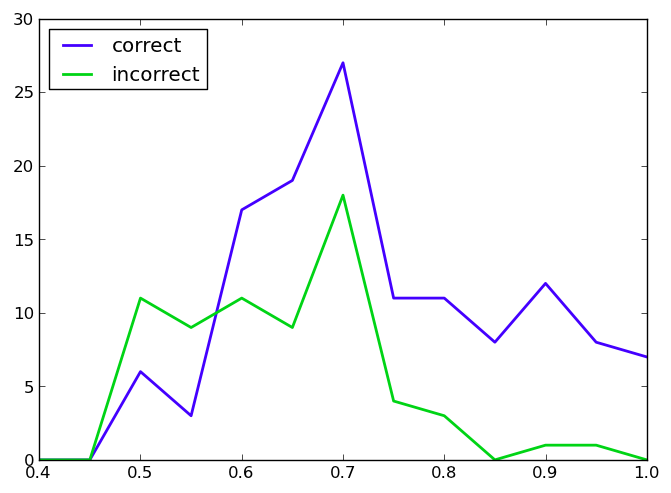
\includegraphics[width=3in]{plots/adam3dist.png}
	\caption{Histogram of ML's for 3 assignments}
\end{subfigure}
&
\begin{subfigure}[b]{3in}
	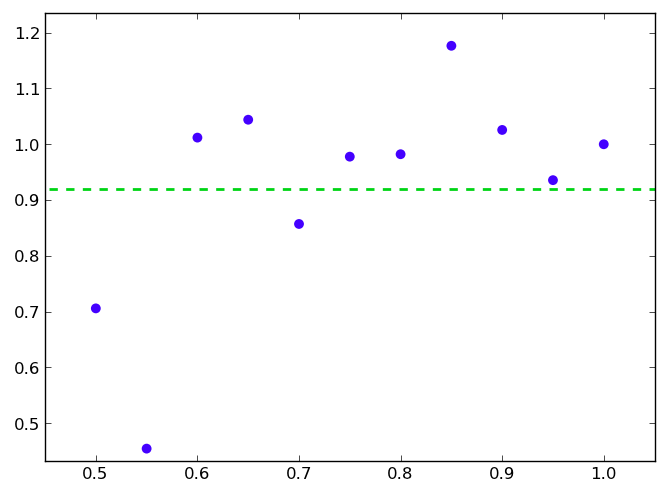
\includegraphics[width=3in]{plots/1adam3.png}
	\caption{Ratio of ML to percentage correct for 3 assignments}
\end{subfigure}
\\
\begin{subfigure}[b]{3in}
	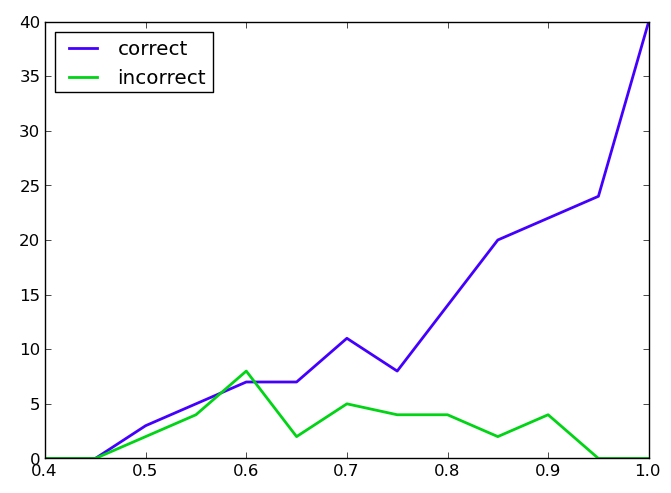
\includegraphics[width=3in]{plots/adam6dist.png}
	\caption{Histogram of ML's for 6 assignments}
\end{subfigure}
&
\begin{subfigure}[b]{3in}
	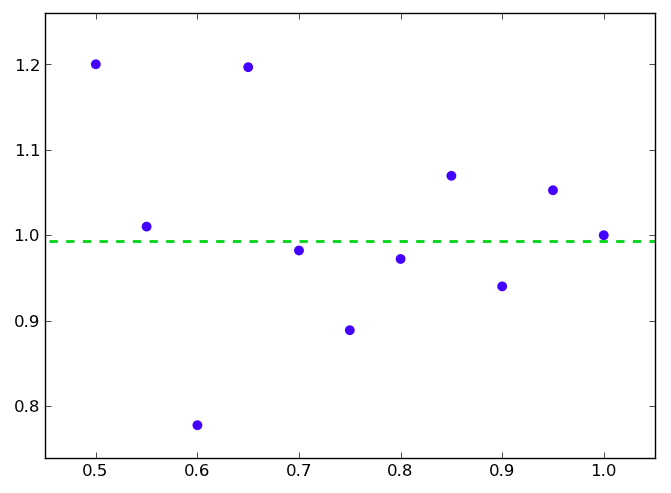
\includegraphics[width=3in]{plots/1adam6.png}
	\caption{Ratio of ML to percentage correct for 6 assignments}
\end{subfigure}
\\
\begin{subfigure}[b]{3in}
	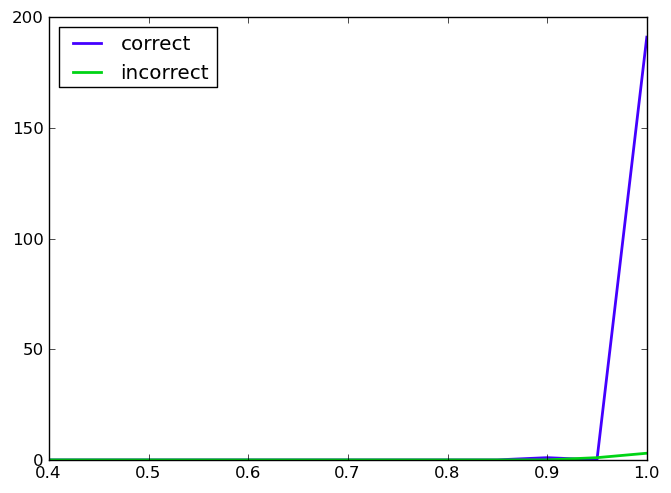
\includegraphics[width=3in]{plots/adam9dist.png}
	\caption{Histogram of ML's for 9 assignments}
\end{subfigure}
&
\begin{subfigure}[b]{3in}
	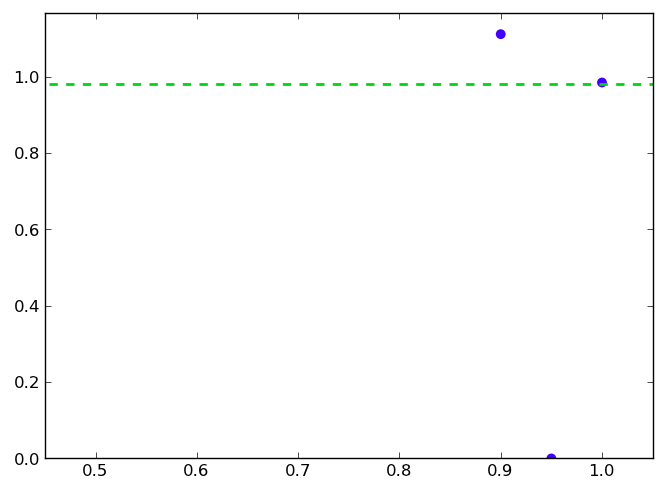
\includegraphics[width=3in]{plots/1adam9.png}
	\caption{Ratio of ML to percentage correct for 9 assignments}
\end{subfigure}
\end{tabular}
\caption{Visualizations of the maximum likelihood values when finding distributions using FCGPE. The left column shows a histogram of students who had a maximum likelihood value (bucketed to 5\%), for both students we could classify correctly and those we couldn't. The right column shows the ratio of the maximum likelihood value to the percentage of students with that value that we could guess correctly. The dotted line show the average, which we want to be close to 1.}
\end{figure*}

\section{Discussion}

\end{document}